\documentclass[12pt,a4paper]{article}
\usepackage[utf8]{inputenc}
\usepackage[T1]{fontenc}
\usepackage{amsmath, amssymb, graphicx, listings, caption}
\usepackage{xcolor}
\usepackage{hyperref}
\hypersetup{
    colorlinks=true,
    linkcolor=blue,
    filecolor=magenta,      
    urlcolor=cyan,
    pdftitle={MNIST Neural Network Report},
    pdfpagemode=FullScreen,
}
\lstset{
    basicstyle=\ttfamily\small,
    backgroundcolor=\color{lightgray!20},
    frame=single,
    keywordstyle=\color{blue},
    commentstyle=\color{green!70!black},
    stringstyle=\color{orange},
    showstringspaces=false,
    breaklines=true,
    tabsize=2,
    numbers=left,
    numberstyle=\tiny,
    numbersep=5pt,
    language=Python
}

\title{\textbf{Detailed Report on Implementing a Neural Network for MNIST Classification}}
\author{Luna Schätzle}
\date{\today}

\begin{document}

\maketitle

\section*{Task Description}
In Task 5, we implemented a neural network to classify the MNIST database. The MNIST database consists of 60,000 training and 10,000 testing images. Each image is $28 \times 28$ pixels, representing a handwritten digit between 0 and 9. The objective was to build a neural network capable of accurately classifying these digits.

The task required implementing a complete workflow, including data preprocessing, designing the neural network architecture, training the model, evaluating its performance, and utilizing the trained model for predictions.

\section*{Data Loading}
The first step was to load the MNIST dataset for use in the model. The function \texttt{load\_data()} was implemented to load the dataset and return the training and test sets.

\subsection*{Code Implementation}
\begin{lstlisting}
import numpy as np
import tensorflow as tf
from tensorflow.keras.datasets import mnist

# Load MNIST dataset
(x_train, y_train), (x_test, y_test) = mnist.load_data()

# Print dataset dimensions
print(f"x_train shape: {x_train.shape}")
print(f"y_train shape: {y_train.shape}")
print(f"x_test shape: {x_test.shape}")
print(f"y_test shape: {y_test.shape}")
\end{lstlisting}

\subsection*{Dataset Analysis}
The MNIST dataset consists of grayscale images, where pixel values range from 0 to 255. To simplify processing for the neural network, pixel values were normalized to the range [0, 1] by dividing by 255. This normalization ensures the neural network can process data efficiently without encountering issues related to large input values.

\subsection*{Visualization}
An example image from the training dataset is displayed below, alongside sample images from each digit category:

\begin{figure}[h!]
    \centering
    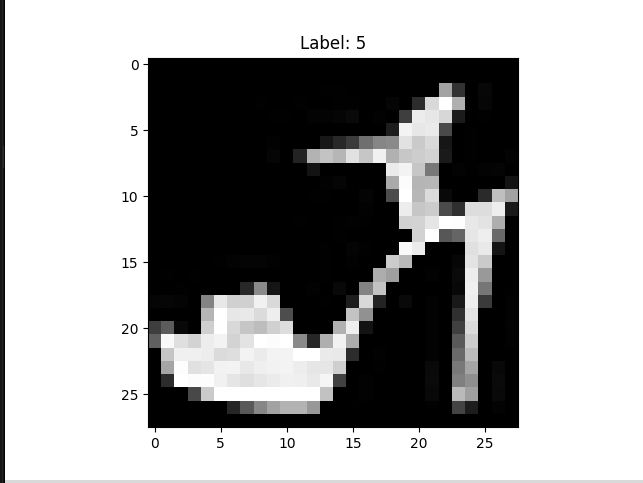
\includegraphics[width=0.6\textwidth]{image-1.png}
    \caption{Example Image from Training Dataset}
    \label{fig:example-image}
\end{figure}

\begin{figure}[h!]
    \centering
    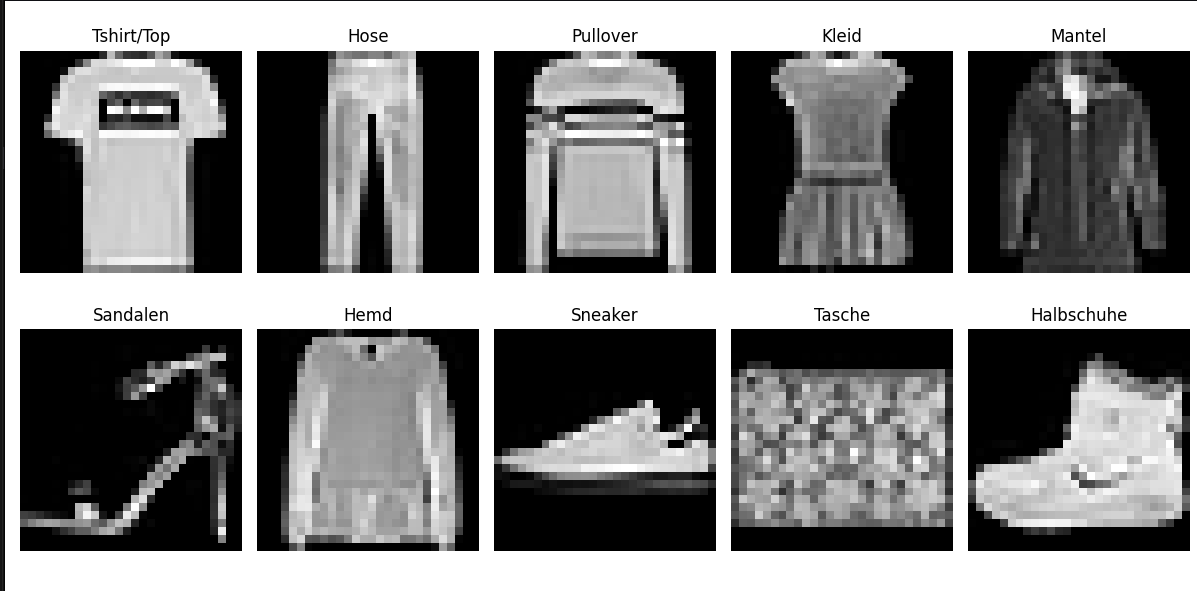
\includegraphics[width=0.8\textwidth]{image-2.png}
    \caption{Sample Images from All Categories}
    \label{fig:sample-images}
\end{figure}

\newpage

\section*{Model Architecture}
The neural network was implemented using Keras. The architecture includes:
\begin{itemize}
    \item An input layer for $28 \times 28$ flattened pixels.
    \item Six dense (fully connected) layers with ReLU activation.
    \item A final output layer with softmax activation for 10 classes.
\end{itemize}

This architecture was chosen to balance simplicity and performance. By stacking multiple layers with decreasing sizes, the model learns progressively abstract features, which aids in accurate classification.

\subsection*{Code Implementation}
\begin{lstlisting}
from tensorflow.keras import models, layers

model = models.Sequential([
    layers.Input(shape=(28 * 28,)),
    layers.Dense(512, activation='relu'),
    layers.Dense(256, activation='relu'),
    layers.Dense(128, activation='relu'),
    layers.Dense(24, activation='relu'),
    layers.Dense(10, activation='relu'),
    layers.Dense(10, activation='softmax')
])
\end{lstlisting}

\subsection*{Model Summary}
\begin{verbatim}
Model: "sequential"
┏━━━━━━━━━━━━━━━━━━━━━━━━━━━━━━━━━┳━━━━━━━━━━━━━━━━━━━━━━━━┳━━━━━━━━━━━━━━━┓
┃ Layer (type)                    ┃ Output Shape           ┃       Param # ┃
┡━━━━━━━━━━━━━━━━━━━━━━━━━━━━━━━━━╇━━━━━━━━━━━━━━━━━━━━━━━━╇━━━━━━━━━━━━━━━┩
│ dense (Dense)                   │ (None, 512)            │       401,920 │
│ dense_1 (Dense)                 │ (None, 256)            │       131,328 │
│ dense_2 (Dense)                 │ (None, 128)            │        32,896 │
│ dense_3 (Dense)                 │ (None, 24)             │         3,096 │
│ dense_4 (Dense)                 │ (None, 10)             │           250 │
│ dense_5 (Dense)                 │ (None, 10)             │           110 │
└─────────────────────────────────┴────────────────────────┴───────────────┘
Total params: 569,600 (2.17 MB)
Trainable params: 569,600 (2.17 MB)
Non-trainable params: 0 (0.00 B)
\end{verbatim}

\section*{Training Process}
The model was trained over 40 epochs using the Adam optimizer and sparse categorical cross-entropy loss. Training and validation accuracy and loss were tracked.

\subsection*{Training Details}
Training involved the following steps:
\begin{enumerate}
    \item Compiling the model with the Adam optimizer and sparse categorical cross-entropy loss.
    \item Splitting data into training and validation sets to monitor performance.
    \item Running the training process for 40 epochs with a batch size of 32.
\end{enumerate}

\subsection*{Training Output}
The training process demonstrated gradual improvements in accuracy and reductions in loss over epochs, as shown in Figure~\ref{fig:training-curves}.

\begin{figure}[h!]
    \centering
    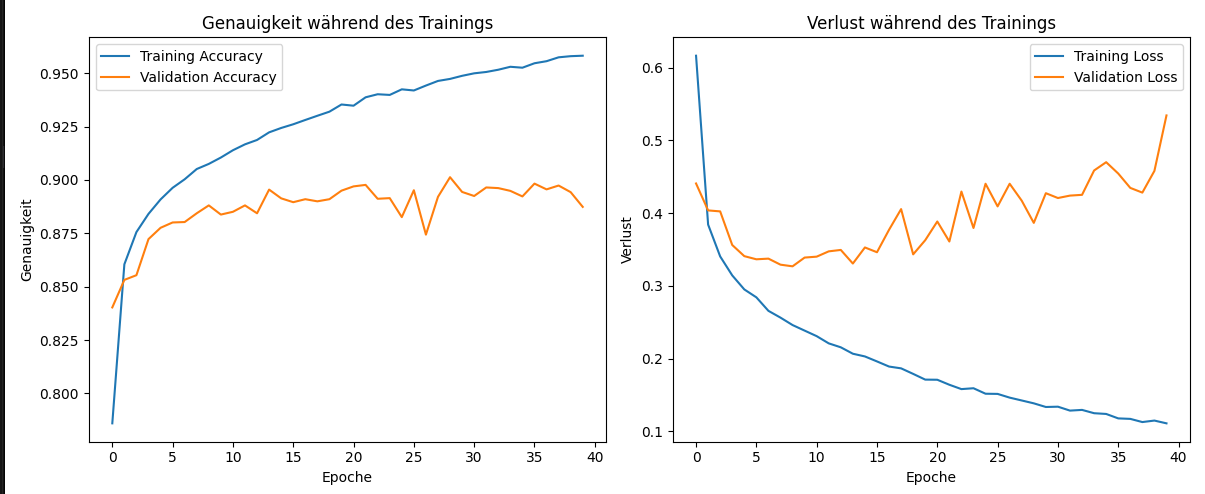
\includegraphics[width=0.8\textwidth]{image.png}
    \caption{Training Accuracy and Loss over Epochs}
    \label{fig:training-curves}
\end{figure}

\section*{Evaluation}
After training, the model was evaluated on the test set. The results were:
\begin{itemize}
    \item Test Loss: 0.5342
    \item Test Accuracy: 88.74\%
\end{itemize}

\subsection*{Performance Insights}
The model achieved high accuracy, indicating effective learning. However, further improvements could involve:
\begin{itemize}
    \item Adding dropout layers to reduce overfitting.
    \item Using convolutional layers to capture spatial relationships.
    \item Tuning hyperparameters such as learning rate and batch size.
\end{itemize}

\section*{Model Usage}
The trained model was saved as \texttt{fashion\_mnist\_model.h5} and can be loaded for predictions. A simple prediction function was implemented to classify images:
\begin{lstlisting}
def predict_image(img_array):
    prediction = model.predict(img_array)
    predicted_class = np.argmax(prediction, axis=1)[0]
    confidence = np.max(prediction) * 100
    return predicted_class, confidence
\end{lstlisting}

\subsection*{Image Preprocessing}
Images must be preprocessed before being passed into the model. Preprocessing includes:
\begin{itemize}
    \item Converting the image to grayscale.
    \item Resizing the image to $28 \times 28$ pixels.
    \item Normalizing pixel values to the range [0, 1].
    \item Flattening the image into a single vector.
\end{itemize}


\begin{figure}[h!]
    \centering
    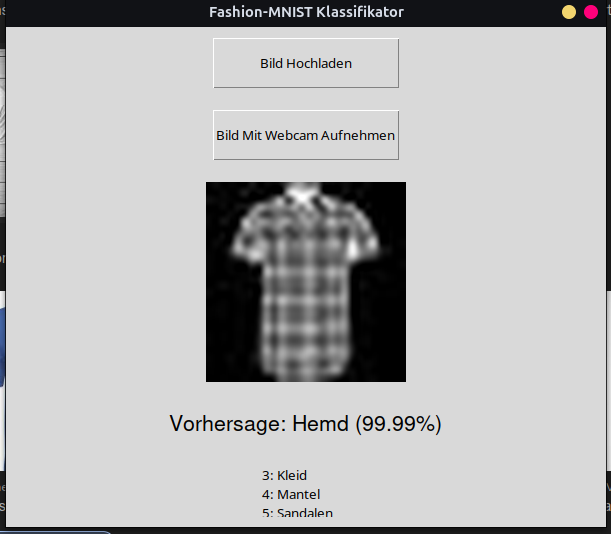
\includegraphics[width=0.8\textwidth]{image-3.png}
    \caption{Implementation of Image Preprocessing and simple User Interface}
    \label{fig:training-curves}
\end{figure}

\section*{Conclusion}
This project successfully implemented a neural network for MNIST digit classification. With a test accuracy of 88.74\%, the model demonstrates reasonable performance. Future improvements could involve hyperparameter tuning, experimenting with convolutional neural networks (CNNs), and increasing the dataset size for enhanced generalization.

\end{document}
